\begin{frame}{Définitions}
    Deux notions développées par Alexandra Saemmer, dans \href{https://shs.cairn.info/revue-communication-et-langages-2020-1-page-99?lang=fr}{\textit{De l’architexte au computexte Poétiques du texte numérique, face à l’évolution des dispositifs}}, 2020:\\
    \begin{itemize}
        \item \textbf{Architexte:} les cases à cocher, les formulaires à remplir, les polices de caractères, couleurs prédéfinies etc...\\
        \textrightarrow{} Contraintes visibles.
        \item \textbf{Computexte:} les contraintes de contenu.
    \end{itemize}
\end{frame}

\begin{frame}{Définitions}
    \begin{block}{}
    On écrit plus dans ces outils mais avec eux. Voire ils écrivent même à notre place.\\
    \textbf{Exemple:} l'auto-complétion.
    \end{block}
    \begin{block}{}
        Rappel exemple des générateurs de texte: l'objectif était de compléter des phrases en appliquant les règles linguistiques.\\
        \textrightarrow{} Les plateformes complètent avec des algorithmes.
    \end{block}
\end{frame}

\begin{frame}{Des dispositifs d'écriture}
    \begin{itemize}
        \item Le nombre de caractères
        \item Le cadre carré d'Instagram
        \item Les émojis sur Facebook
    \end{itemize}
\end{frame}

\begin{frame}{Exemple: la Broetry sur LinkedIn}
    \begin{columns}
    % Colonne de gauche : Texte
        \begin{column}{0.4\textwidth}
            \begin{itemize}
                \item Billet de blog de Carina Rampelt (\url{https://fenwick.media/rewild/magazine/dead-broets-society-behind-the-strange-story})
                \item Forme de storytelling sur LinkedIn
                \item Pousser les gens à cliquer sur "voir plus", ce qui signale à LinkedIn que vous êtes intéressées
            \end{itemize}
        \end{column}

        % Colonne de droite : Image
        \begin{column}{0.5\textwidth}
            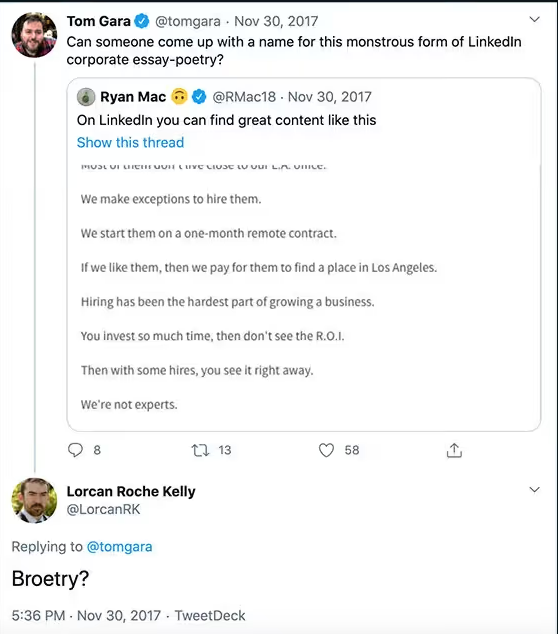
\includegraphics[width=.9\columnwidth]{Images/Broetry.png}
            
        \end{column}
    \end{columns}
\end{frame}

\begin{frame}{Exemple: la Broetry sur LinkedIn}
    Carina Rampelt décrit les règles de la Broetry comme suit:
    \begin{itemize}
        \item Une phrase d'ouverture "\textit{click bait}"
        \item Le contenu: une anecdote personnelle
        \item Le format: court, phrase simple avec des sauts de ligne 
        \item La phrase de conclusion: une leçon de vie cliché ou "\textit{inspirational quote}"
    \end{itemize}
\end{frame}

\begin{frame}{Exemple: la Broetry sur LinkedIn}
    \centering
    
\includegraphics[width=.6\textwidth]{Images/broetry_regles.png}
\end{frame}